\section{Recovering a Certificate Before a Nonlinear ReLU Suffix}\label{sec:nonlinear-application}
The first application fixes the whole network, input region and merge policy. Changing the diagonal representative alone recovers the \emph{exact} classification margin. The suffix is nonlinear at the hidden-state cut, so the affine zero-loss result in dimension two does not apply.

\paragraph{Network and specification.}
For $t\in[0,3]$, let $\sigma(s)=\max(0,s)$ and
\begin{align*}
F_1(t)&=\sigma(t-1)-\tfrac74\sigma(t-2),\\
F_2(t)&=\tfrac34-\tfrac34\sigma(t)+\tfrac74\sigma(t-1)-\sigma(t-2).
\end{align*}
The hidden image traverses $(0,3/4)\to(0,0)\to(1,1)\to(1/4,1)$. It is $R=V\cup D_2\cup H$, where $V=\{(0,s):0\le s\le3/4\}$ and $H=\{(s,1):1/4\le s\le1\}$. The prefix uses one width-three ReLU layer and a width-two affine/ReLU layer; the latter ReLU is the identity on $K_2$.

Put $z^\star=(1/4,3/4)$ and take logits $g_1(z)=\norm{z-z^\star}$, $g_2(z)=1/8$. An explicit standard ReLU suffix computes
\[
h=(\sigma(z_1-1/4),\sigma(1/4-z_1),\sigma(z_2-3/4),\sigma(3/4-z_2)),
\]
then $k_1=\sigma(h_1+h_2-h_3-h_4)$, $k_2=\sigma(h_3+h_4)$, and $g_1=k_1+k_2$. Thus the full architecture is $1\to3\to2\to4\to2\to2$, with an affine output. Since $\dist_\infty(z^\star,R)=1/4$, its true minimum margin $\psi=g_1-g_2$ is $1/8$.

\paragraph{Fixed merge interface.}
Split the input at $1$ and $2$ and represent all three hidden segments exactly. For the axial segments use
\begin{align*}
U_V&=\Hu\{E(0,0),E(0,3/4),(0,0,0,-3/4)\}=V\times(-V),\\
U_H&=\Hu\{E(1,1),E(1/4,1),(1/4,1,-1,-1)\}=H\times(-H).
\end{align*}
For the diagonal use either $P_3=\Hu\{E(0),E(\one_2),c(0,1)\}$ or
\[
P_4=\Hu\{E(0),E(\one_2),c(0,1/2),c(1/2,1)\},\qquad
c(a,b)=(a,a,-b,-b).
\]
The merged state is $A_i=K_2\cap E^{-1}\Hu(P_i\cup U_V\cup U_H)$. Evaluate the suffix exactly on this state; additional suffix-relaxation error is outside this comparison.

\begin{proposition}[Exact certificate recovery]\label{prop:nonlinear-recovery}
The true minimum margin is $1/8$, while $\min_{A_3}\psi=-1/8$ and $\min_{A_4}\psi=1/8$. Every exact diagonal representative with at most three finite generators fails for this fixed interface. Four diagonal generators suffice and are minimal. After shared endpoints are counted once, the displayed full merge lists contain seven and eight generators, respectively; no minimality of that total is claimed.
\end{proposition}
\begin{proof}
Let $g=c(0,1)$ and $p=(1/4,1/4,-3/4,-3/4)$. We have
\begin{align*}
p&=\max\{g,E(0)-\tfrac34\one_4,E(\one_2)-\tfrac34\one_4\}\in P_3,\\
E(z^\star)&=\max\{p,E(1/4,1)-\tfrac14\one_4,E(0,3/4)-\tfrac14\one_4\}.
\end{align*}
Both combinations are normalized, so $z^\star\in A_3$. Since $\psi\ge-1/8$ everywhere, this gives the exact abstract minimum. Theorem~\ref{thm:partition} places $P_3$ inside every admissible three-generator diagonal representative, preserving the witness.

A normalized combination yielding $E(x)\in\Hu(P_4\cup U_V\cup U_H)$ has a coefficient-zero generator dominated by $E(x)$. For the two refined diagonal anchors this forces $x\in[0,1/2]^2$ or $[1/2,1]^2$. For the axial anchors it forces $x\in V$ or $H$; a consistent endpoint forces equality to that endpoint. Thus
\[
A_4\subseteq V\cup H\cup[0,1/2]^2\cup[1/2,1]^2.
\]
Every point in this cover is at distance at least $1/4$ from $z^\star$: on the lower square use coordinate two, on the upper square coordinate one, and on $V,H$ their fixed coordinates. Hence $\psi\ge1/8$. The reachable diagonal point $(1/2,1/2)$ attains this bound. Budgets below three cannot represent the diagonal, completing minimality.
\end{proof}

\begin{figure}[t]
\centering
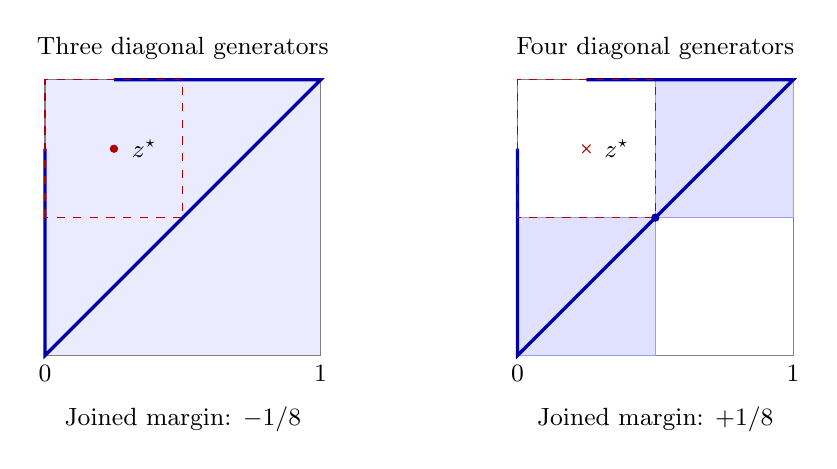
\begin{tikzpicture}[x=3.5cm,y=3.5cm,font=\small]
\begin{scope}
\fill[blue!8] (0,0) rectangle (1,1);
\draw[gray] (0,0) rectangle (1,1);
\draw[very thick,blue!65!black] (0,.75)--(0,0)--(1,1)--(.25,1);
\draw[red!70!black,dashed] (0,.5) rectangle (.5,1);
\fill[red!70!black] (.25,.75) circle (1.5pt);
\node[right] at (.28,.75) {$z^\star$};
\node[below] at (0,0) {$0$};\node[below] at (1,0) {$1$};
\node[above] at (.5,1.04) {Three diagonal generators};
\node[below] at (.5,-.15) {Joined margin: $-1/8$};
\end{scope}
\begin{scope}[xshift=6.0cm]
\fill[blue!12] (0,0) rectangle (.5,.5);
\fill[blue!12] (.5,.5) rectangle (1,1);
\draw[gray] (0,0) rectangle (1,1);
\draw[blue!40] (0,0) rectangle (.5,.5);
\draw[blue!40] (.5,.5) rectangle (1,1);
\draw[very thick,blue!65!black] (0,.75)--(0,0)--(1,1)--(.25,1);
\draw[red!70!black,dashed] (0,.5) rectangle (.5,1);
\draw[red!70!black] (.235,.735)--(.265,.765) (.235,.765)--(.265,.735);
\node[right] at (.28,.75) {$z^\star$};
\fill[blue!65!black] (.5,.5) circle (1.5pt);
\node[below] at (0,0) {$0$};\node[below] at (1,0) {$1$};
\node[above] at (.5,1.04) {Four diagonal generators};
\node[below] at (.5,-.15) {Joined margin: $+1/8$};
\end{scope}
\end{tikzpicture}

\caption{The blue path is the same exact reachable set in both panels. Shading shows the diagonal anchors' necessary cover for consistent joined states, not the exact joined set; the axial operands add $V$ and $H$. The dashed square has radius $1/4$ about $z^\star$. The refined cover avoids its interior, certifying the distance margin.}\label{fig:recovery}
\end{figure}

\paragraph{Meaning of the intervention.}
The refined anchors replace the coarse anchor; simply adjoining generators would retain its spurious state. The guarantee concerns exact suffix evaluation on the merged set, not the bounds of an unspecified heuristic solver. Querying the three regions separately or retaining their disjunction also certifies the network. Reusable hidden-state summaries are a possible reason to merge, but neither reuse nor partitioning is new~\cite{fischer2021,singh2019}. The example demonstrates a representation choice at that interface; its frequency and cost on trained models are empirical questions.

The axial representatives above behave like their concrete segments even in arbitrary ambient joins. Appendix~\ref{app:neural-transfer} proves this fact and uses safe axial connectors to realize worst affine and Lipschitz contextual losses by continuous ReLU networks. The realizing network may depend on the representative, and connector storage is an additional resource. Section~\ref{sec:relu-application} gives a distinct affine-readout contract; its positive lower bound is not claimed to recover the exact margin.
